\chapter{Non-Relational Database} 

Relational database has been introduced in the earlier chapter. This chapter discusses non-relational database.

\section{Brief Introduction to Non-Relational Database}

Non-relational database (NoSQL database) emerged in $2000$s. In contrast to RDBMS, NoSQL databases do not store data in tables but in key-value pairs, graphs, documents, or other formats.

Though it may not be as intuitive as RDB, NoSQL database can become more efficient and easier to use in some applications. For example, NoSQL databases can be very fast in query, and are becoming popular in handling big data in real-time web applications. However, many non-relational databases compromise consistency issue, and can only provide ``eventual consistency'' but not ``strong consistency''. This implies that the latest update in the database may not be reflected in an immediate query. Examples of NoSQL databases include \textit{Redis}, \textit{Azure Cosmos DB}, \textit{Oracle NoSQL Database}, \textit{Amazon DynamoDB} and \textit{AllegroGraph}.

Unlike SQL which applies to almost all RDB, there is no universally adopted language for NoSQL databases. Each NoSQL database often has its unique query language tailored to its specific data model. We use ``NoSQL'' to refer to a collective set of languages used for NoSQL database management. For basic SQL applications, different RDB may perform similarly, with some subtle differences in the performance. However, this is not the sime with NoSQL databases. Different NoSQL databases may look and function completely differently even for the most simple applications.

Database services, both RDB and NoSQL, have become critical to our daily life and they are massively deployed on servers. In many applications they work together to deliver the service.

\section{Non-RDB Example: MongoDB}

Unlike relational databases where data is stored in relevant tables with pre-designed schematics such as column names, types, and references, non-relational database stores data in different structures such as directed graphs, dictionaries and documents.

Though relational databases are intuitive and came early in time, non-relational databases are also spreading, as in some occasions they can be easier to use and can be more flexible and powerful. For example, some NoSQL databases are more effective when dealing with massive parallel requests, handling large data, and providing highly scalable and available services.

There are many types of non-relational databases including document-oriented databases, directed graph databases, etc., Each of them has some unique features, pros and cons over other databases, and may adopt its own database manipulation language. It is impossible to cover everything in this notebook. Only brief introductions of selected databases examples are given here. More details might be found on other relevant notebooks, for example graphical database in \textit{A Notebook on Probability, Statistics and Data Science}.

MongoDB is a source-available cross-platform document-oriented database program. Classified as a NoSQL database program, MongoDB uses JSON-like documents with flexible schemas. This is not surprising, as MongoDB has a close connection with JavaScript. It is powered by a JavaScript engine. MongoDB, together with other JavaScript-relevant software such as \textit{Express.js}, \textit{React.js}, \textit{Node.js}, etc., can be used to create database-powered web applications.

Comparing with conventional RDBs, MongoDB is more capable at
\begin{itemize}
	\item Massive data storage (in the order of TBs and PBs);
	\item Frequent and parallel operations such as insert and query;
	\item Flexible scalability and high availability.
\end{itemize}
Notice that MongoDB as well as many other NoSQL databases are not suitable to handle financial transactions due to the consistency issue that many NoSQL databases suffer. But things might change as new technologies emerge.
Examples of scenarios that MongoDB can be used include
\begin{itemize}
	\item Posts and streaming management on social media websites or APPs;
	\item Online gaming information storage;
	\item Logistics industry and supply chain management;
	\item IoT data management.
\end{itemize}

As a document-oriented database, MongoDB stores data not in relational tables, but in separated collections (corresponding with tables) and documents (corresponding with rows). Each document in the same collection can adopt its own schema. When querying data, the user does not need to join collections and map documents. Figure \ref{ch:database:mongotree} is given as a demonstration of how MongoDB stores and organizes data.
\begin{figure}[htbp]
	\centering
	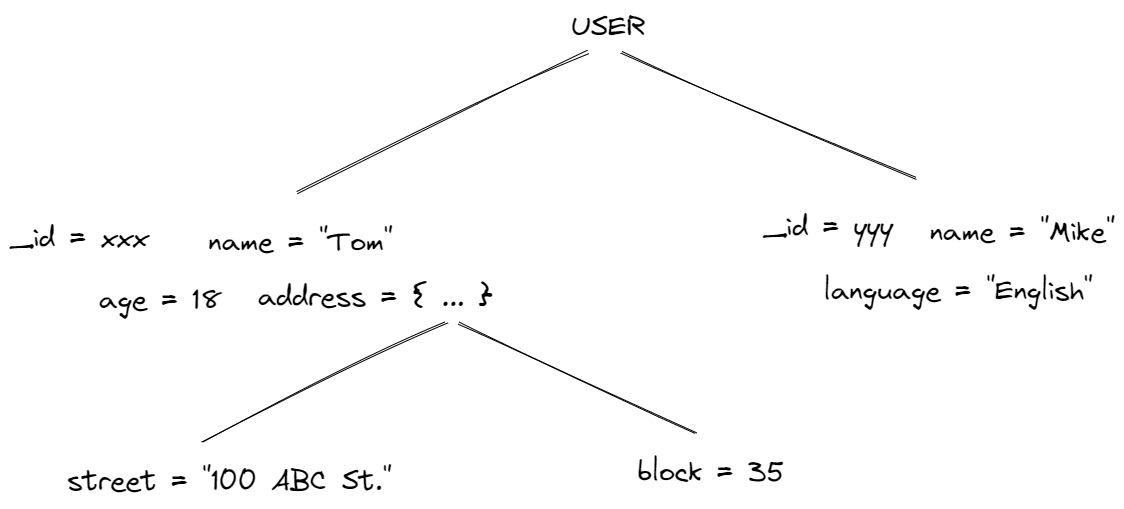
\includegraphics[width=250pt]{chapters/part-3/figures/mongodb_tree.png}
	\caption{A demonstration of MongoDB storing data as object-of-object.} \label{ch:database:mongotree}
\end{figure}

In Fig. \ref{ch:database:mongotree}, a collection ``USER'' is defined. The collection contains two documents. Each document has a few properties. Different document may share common properties such as ``name'' in this example. Each of them can also have unique properties of its own such as ``age'', ``address'' and ``language''. Different properties may have different data types. For example, a property can be string, numeric, or an object, or a list of the above. When querying MongoDB, the DBMS is able to return selected properties of documents that meet specific criteria, and sort them in required order.

\subsection{Installation}

MongoDB, like many other DBMS, has both community and enterprise versions. MongoDB community server can be installed following the instructions in the official website
\begin{lstlisting}
https://www.mongodb.com/try/download/community
\end{lstlisting}
To interact with MongoDB DBMS, the quickest way is to use MongoDB shell (also known as ``mongosh''). A description of the shell can be found at
\begin{lstlisting}
https://www.mongodb.com/try/download/shell
\end{lstlisting}
Notice that when installing MongoDB server, it is possible that the server comes with MongoDB Compass, the GUI for MongoDB DBMS. The GUI can also be used to interact with the databases.

Different versions of MongoDB are available. Choose the correct MongoDB version depending on the CPU and the OS of the machine. MongoDB community server installation size is about 500MB.

MongoDB provides enterprise service, MongoDB Atlas, as part of its cloud solution where user can deploy clusters to host databases. With proper gateway setup, the user can connect to MongoDB Atlas clusters from his local server to retrieve data or to manipulate the databases. MongoDB Atlas is not the covered in this notebook.

\subsection{Basic Global Operations}

After installing both MongoDB server and MonghDB shell, use
\begin{lstlisting}
$ mongosh
\end{lstlisting}
in the command line to login to the DBMS. JavaScript-like commands are used to manipulate the database, including creating databases and inserting data.

The object \verb|db| contains many methods using which the user can access and modify the basic configurations of the database. For example,
\begin{lstlisting}
> db.version()
\end{lstlisting}
gives the version of the database server. More commands can be found using \verb|db.help()|. Some commonly used commands are listed in Table \ref{ch:db:tab:mongodbbasics}.
\begin{table}
	\centering \caption{MongoDB basic commands.}\label{ch:db:tab:mongodbbasics}
	\begin{tabularx}{\textwidth}{lX}
		\hline
		Command & Description \\ \hline
        \verb|db.help()| & Show a list of methods of \verb|db| object. \\ \hdashline
		\verb|db.version()| & Show database server version. \\ \hdashline
        \verb|db.getUsers()| & Show users. \\ \hdashline
        \verb|db.createUser(<content>)| & Create a user. The username, password, roles, etc., needs to be included in the \verb|<content>| area. \\ \hdashline
        \verb|db.dropUser(<username>)| & Drop a user. \\ \hdashline
        \verb|db.dropDatabase()| & Drop current database. \\ \hdashline
		\verb|db.status()| & Show the basic status of the currently selected database, such as its name, number of collections, storage size, etc.  \\ \hdashline
        \verb|db.getUsers()| & Show users. \\
		 \hline
	\end{tabularx}
\end{table}

To display the existing databases, use
\begin{lstlisting}
> show dbs
\end{lstlisting}
On a clean installation, the above should return the 3 default databases, \verb|admin|, \verb|config| and \verb|local|. To change to a particular database, use
\begin{lstlisting}
> use <database_name>
\end{lstlisting}
Notice that there is no ``create database'' command in MongoDB. To create a database, switch to that database using the above command (even though it does not exist yet), and create some data such as a collection there. The database will be automatically created. This is again a feature closely related to JavaScript.

\subsection{Data Format}

MongoDB is a document-oriented database program. The data is stored in the format of ``binary JSON'' (BSON), which can be taken as an extension of JSON that supports more data types. Since BSON and JSON have a strong connection to the JavaScript object datatype, which looks very similar to a ``dictionary'', one may claim that MongoDB uses key-value pairs to store data. That statement is partially correct because BSON indeed adopts key-value pair structure to store data, but it may over simplifies the reality and be misleading sometimes. In fact, BSON supports much more complicated data types other than string-to-string, such as array and nested objects.

JSON supports 6 datatypes: number, string, boolean (true or false), object, array and null. Notice that JSON is text-based, which is essentially a string. It is a notation of data. It does not concern how the data would be stored and used in the program that takes JSON as the input file. For example, from JSON's point of view, it does not distinguish different types of number, being integer or float or double. In JSON, it is just a notation of number, say ``$108$''. It is the program's responsibility to decide how to treat the number, either as an integer, or as a 32-bit float, or a 64-bit float.

BSON, on the other hand, is binary-based, which is essentially a list of binary numbers. This makes BSON more efficient (but less flexible and more difficult to use sometimes) than JSON. In BSON, more datatypes are supported, including: double (64-bit float), string, object, array, binary data (a binary string), object id, boolean, date, null, regular expression, JavaScript code, 32-bit integer, 64-bit integer, timestamp, etc. When using BSON, the user needs to be more specific on how the data should be stored. For example, for a number ``$108$'', the user needs to specify whether to store it as a 32-bit integer or a 64-bit integer, or maybe as a 64-bit float.

Both JSON and BSON are intuitive and human-readable. MongoDB uses BSON due to its enhanced capability.

\subsection{Create Collection and Document}

A MongoDB database contains multiple collections. A collection is similar to a table in an RDB in the sense that it is the ``host'' of similar data. However, unlike tables where schematics such as column names and datatypes are enforced upon creation of the table, a collection does not enforce fields and data types. An example of creating a collection inside a database is given below.
\begin{lstlisting}
> use testdb;
> db.createCollection("users");
\end{lstlisting}
Use \verb|show collections| to show the collections in the current database.

\begin{shortbox}
\Boxhead{Should I use semicolon in the end of each MongoDB command?}

If you are using MongoDB shell, then technically speaking, you don't have to. It works both ways. However, if you are using JavaScript environment such as \textit{Node.js} and integrating MongoDB commands as part of the program, you should use semicolon.

For example, to create a new database, in MongoDB shell
\begin{lstlisting}
> use myNewDatabase
\end{lstlisting}
or
\begin{lstlisting}
> use myNewDatabase;
\end{lstlisting}
would both work just fine. However, in \textit{Node.js},
\begin{lstlisting}
const newDb = client.db("myNewDatabase");
\end{lstlisting}
the semicolon is required.

As a conclusion, semicolon is recommended mostly, just to follow the general JavaScript good practice. Although in JavaScript semicolon is also optional due to Automatic Semicolon Insertion (ASI), it is still widely recommended to use semicolon anyway.
\end{shortbox}

Data can be installed into a collection. An entry to be inserted to a collection, corresponding with a row of a table in RDB, is called a document. It is possible to insert one or multiple entries at a time. To insert documents, first prepare the document in BSON format. For example, consider the following documents.
\begin{lstlisting}
{
  name: "Alice",
  age: 20,
  address: "123 Center Park",
  hobbies: ["football", "reading"],
  parents: {
    father: "Chris",
    mother: "Kite"
  }
}

{
  name: "Bob",
  age: Long.fromNumber(25),
  address: "135 Center Park",
  hobbies: BSON.Array(["basketball", "jogging"])
}
\end{lstlisting}
Notice that user ``Alice'' and ``Bob'' are represented by JSON and BSON, respectively. MongoDB uses BSON internally, but it can also take JSON as input, in which case MongoDB driver converts JSON to BSON.

Then use the following syntax to insert the document into the collection.
\begin{lstlisting}
db.<collection_name>.insertOne({...});
db.<collection_name>.insertMany([{...}, {...}, {...}]);
\end{lstlisting}
where \verb|{...}| is the document in JSON or BSON format as shown earlier. To make it more readable, consider do the following instead.
\begin{lstlisting}
const doc = {...};
db.<collection_name>.insertOne(doc);
\end{lstlisting}
which first store the document in \verb|doc|, then pass it to \verb|insertOne()| method. Upon successful insertion, an insert id (also known as object id) will be created automatically.

\subsection{Query}

MongoDB uses \verb|find({...})|, \verb|findOne({...})| to find documents, where \verb|{...}| is a query argument in the form of JavaScript object. Details are given below.

To obtain all the document under a collection, use
\begin{lstlisting}
db.getCollection('<collection_name>').find({});
\end{lstlisting}
where an empty query simply matches all documents in the collection. Of course, when \verb|findOne()| is used, it will return only one document. When an object is given in the query, MongoDB returns only the documents containing the same fields.

Notice that
\begin{lstlisting}
db.collection_name.some_function()
\end{lstlisting}
is equivalent with
\begin{lstlisting}
db.getCollection('<collection_name>').find({});
\end{lstlisting}
The first implementation is more convenient while the second more flexible as it supports dynamic naming, i.e., something like
\begin{lstlisting}
collectionName = 'some_collection';
db.getCollection(collectionName).some_function();
\end{lstlisting}

Several examples are given below. To find documents that has a certain field with certain values, use the following
\begin{lstlisting}
db.getCollection('posts').find({comments: 1})
\end{lstlisting}
The above query search documents with field \verb|comments| whose value is $1$ under collection \verb|posts|. To get those posts with at least $1$ comment, use the following
\begin{lstlisting}
db.getCollection('posts').find({comments: {$gt: 0}})
\end{lstlisting}
where \verb|{$gt: 0}| stands for any value greater than $0$. Commonly seen query operators are given in Table \ref{ch:db:tab:mongodbqueryoperator}, each with an example.

\begin{table}
	\centering \caption{MongoDB basic query operators.} \label{ch:db:tab:mongodbqueryoperator}
	\begin{tabularx}{\textwidth}{llX}
		\hline
		Operator & Description & Example \\ \hline
		\verb|$gt| & Greater than & \verb|{age: {$gt: 18}}| \\ \hdashline
		\verb|$lt| & Less than & \verb|{age: {$lt: 18}}| \\ \hdashline
		\verb|$and| & And & \verb|{$and: [{age: {$gt: 18}}, {sex: 'M'}]}| \\ \hdashline
		\verb|$or| & Or &  \verb|{$or: [{age: 18}, {age: 21}]}| \\ \hdashline
		\verb|$in| & In & \verb|{name: {$in: ['Alice', 'Bob']}}| \\ \hdashline
		\verb|$nin| & Not in & \verb|{name: {$nin: ['Alice', 'Bob']}}| \\
		\hline
	\end{tabularx}
\end{table}

\subsection{Update and Remove Document}

Two functions, \verb|updateOne(...)| and \verb|updateMany(...)|, are provided to update documents. Details are given below via an example.
\begin{lstlisting}
db.getCollection('users').updateOne(
	{userId: '0015'},
	{$set: {age: 25}}
);
\end{lstlisting}
The above code query \verb|users| collection, find the document with \verb|userId| being \verb|'0015'|, and change its \verb|age| field to $25$. From this example, it can be seen that the document updating function contains a query and a set of updating operators. Commonly seen updating operators are given in Table \ref{ch:db:tab:mongodbupdateoperator}.

\begin{table}
	\centering \caption{MongoDB basic update operators..}\label{ch:db:tab:mongodbupdateoperator}
	\begin{tabularx}{\textwidth}{lX}
		\hline
		Operator & Description \& Example \\ \hline
		\verb|$set| & Replace field value \\ & \verb|{<query>}, {$set: {age: 30 } }| \\ \hdashline
		\verb|$unset| & Remove field \\ & \verb|{<query>}, {$unset: {age: ""} }| \\ \hdashline
		\verb|$inc| & Increment a field by a value \\ & \verb|{<query>}, {$inc: {age: 1} }| \\ \hdashline
		\verb|$rename| & Rename field \\ &  \verb|{<query>}, {$rename: {"age": "yearsOld"}}| \\ \hdashline
		\verb|$currentDate| & Set field value to current date \\ & \verb|{{<query>}, {$currentDate: {lastModified: true}}}| \\ \hdashline
		\verb|$addToSet| & Add element to array field \\ & \verb|{<query>}, {$addToSet: {hobbies: "reading"}}| \\
		\hline
	\end{tabularx}
\end{table}

Use either \verb|deleteOne({<query>})| or \verb|deleteMany({<query>})| to remove documents.

\subsection{Sharding and Indexing}

Given that MongoDB is often used with massive data storage, efficient query from massive storage becomes critical. MongoDB implements a few technologies to speed up the query, including sharding and indexing.

Sharding is a method of distributing data across multiple servers or instances. In MongoDB, a shard consists of a subset of the total dataset, and each shard is responsible for managing a portion of the data. This distribution allows MongoDB to scale horizontally by adding more servers, thereby spreading the load and the data volume across a cluster. When a query is executed, it only needs to be processed by the shards that contain relevant data, rather than the entire dataset. This can significantly reduce query times in a large, distributed system. Sharding is particularly useful for very large datasets and high throughput operations, where a single server would not be sufficient to store the data or provide acceptable performance.

Indexing is a technique used to speed up the retrieval of documents within a database. MongoDB uses indexes to quickly locate data without having to scan every document in a collection. Indexes are a critical component of database optimization, as they can drastically reduce the amount of data MongoDB needs to look through to find documents that match a query.

MongoDB primarily uses B-Tree data structures for its indexes. A B-Tree is a self-balancing tree data structure that maintains sorted data in a way that allows searches, sequential access, insertions, and deletions in logarithmic time. The ``B'' in B-Tree stands for ``balanced'' and indicates that the tree is designed to keep the data balanced, ensuring that operations are efficient even as the dataset grows. The B-Tree structure allows MongoDB to perform efficient searches. Instead of scanning every document in a collection, MongoDB can use the B-Tree index to quickly navigate through a small subset of the data to find the documents that match the query criteria.

There are many ways to define the index. For example, it is possible to use a single field to form a single field index, or to use multiple fields to form a compound index. Index by itself is also an argumented data structure and it consumes disk space. Each time there is a write operation, the index needs to be updated. Therefore, a very complicated index schema slows down data insertion. It is critical to design appropriate index to optimize the overall performance of the database.

MongoDB provides commands to check, set and remove indexes. To check the indexes of a system, use
\begin{lstlisting}
db.collection_name.getIndexes()
\end{lstlisting}

\subsection{Other Features}

MongoDB uses aggregation framework provides way to perform complex data transformations in a ``pipeline''. The data is processed step-by-step.

When a document is added to a collection, a default field \verb|_id| is added. Querying via \verb|_id| is usually faster than with other criteria because otherwise MongoDB has to search for the entire collection to find relevant documents. 

Data in MongoDB can be exported or imported from files, such as BSON and JSON files.

MongoDB, like many other DBMS especially cloud-based enterprise tier ones, provide replica setting to tackle read-heavy applications. A primary server is replicated to multiple replicas. Writing is allowed only to the primary server, but reading is allowed to all replicas as well as the primary server. In the case of MongoDB, when primary server fails, one of the replicas is automatically promoted to be the primary server.

\section{Non-RDB Example: MongoDB Atlas}

MongoDB Atlas is the MongoDB cloud-based serverless solution. It allows the user to deploy MongoDB on the cloud. The user has the freedom to choose the base cloud service provider(s) including AWS, Azure and Google Cloud, and more. Thanks to Altas, the user has the flexibility to seamlessly change cloud service providers and service tiers without downtime. 

In addition to just a host of the database, Atlas provides varieties of tools that helps the developer to develop applications using the database, such as a centralized cloud-based dashboard, autonomous synchronization with edge devices, etc. Some other examples include Atlas data lake which optimized for analytical queries. Big data can be stored in Atlas data lake, from where analytical information can be retrieved. Atlas federation allows seamlessly query, transform, and aggregate data from one or more MongoDB Atlas databases and cloud object storage offerings. Atlas chart provides rich tools for MongoDB data visualization. There are many more tools.

As of this writing, Atlas allows the user to choose from 3 different storage tiers:
\begin{itemize}
  \item Shared: the database is stored on shared servers; the user can select the server provider from AWS, Azure and Google Cloud
  \begin{itemize}
    \item M0: free, $512$MB
    \item M2: 2GB, \$$9$ / month
    \item M5: 5GB, \$$25$ / month
  \end{itemize}
  \item Dedicated: the database is stored on dedicated servers with dedicated storage, RAM and multi-core CPUs; $10$GB to $4$TB; \$$0.08$ / hour - \$$33.26$ / hour
  \item Serverless: the database is provided as a microservice, and it automatically scales up and down based on use; up to 1TB; the cost depends on the amount of stored data, the number of read and write operations, the computational cost of backups, etc.
\end{itemize}

\subsection{Create a Database}

To use MongoDB Atlas, register an account with MongoDB Atlas. Create a database. Select the pricing tier for the database, create a user with admin role and assign him a password, and configure the database access gateway (i.e., a list of IP address that can access the database).

The created database is emply. For tutorial purpose, Altas provides a sample database. One can import the data in the sample database into the created empty database. MongoDB Atlas dashboard provides data explorer tool that allows the user to view and edit the database (in the form of JSON documents) directly, without using CLI or code. One can also filter documents from a collection by filtering the fields of the documents.

The following screenshot in Fig. \ref{ch:database:atlasdashboard} gives MongoDB Atlas dashboard, after the sample data has been imported. The database, database access (user) and network access (gateway) can be accessed from the dashboard.

\begin{figure}[htbp]
	\centering
	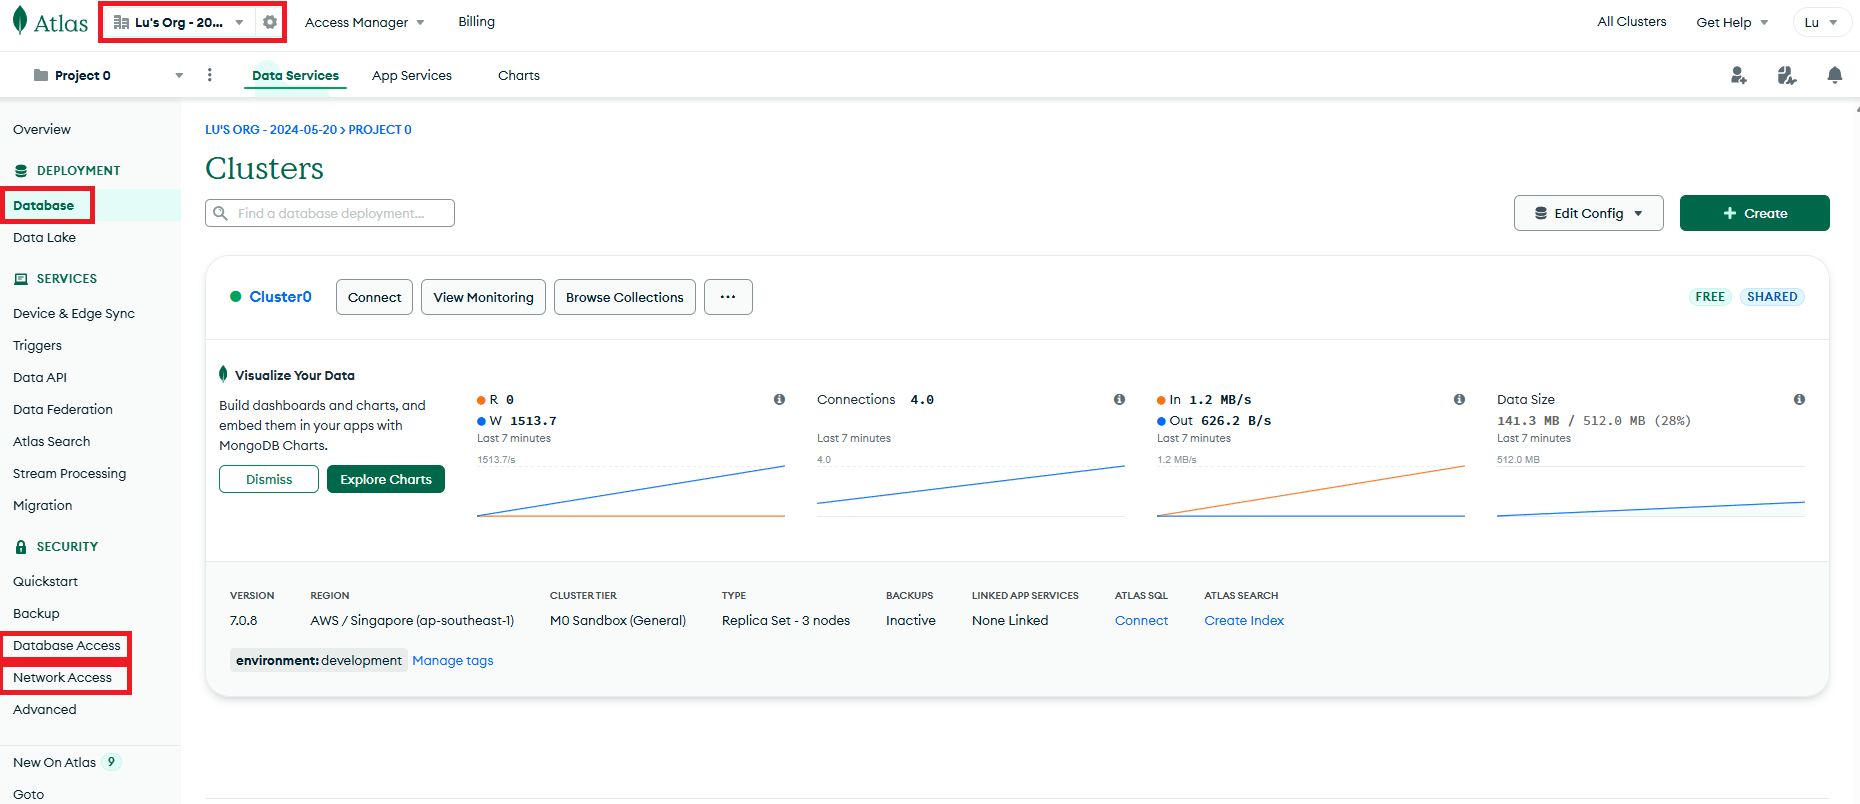
\includegraphics[width=\textwidth]{chapters/part-3/figures/atlas_dashboard.png}
	\caption{A demonstration of MongoDB Atlas dashboard.} \label{ch:database:atlasdashboard}
\end{figure}

Click ``Browse Collections'' of the cluster in Fig. \ref{ch:database:atlasdashboard}. This sample database cluster contains multiple databases, each database with several collections, as shown by Fig. \ref{ch:database:atlasdashboard2}.

\begin{figure}[htbp]
	\centering
	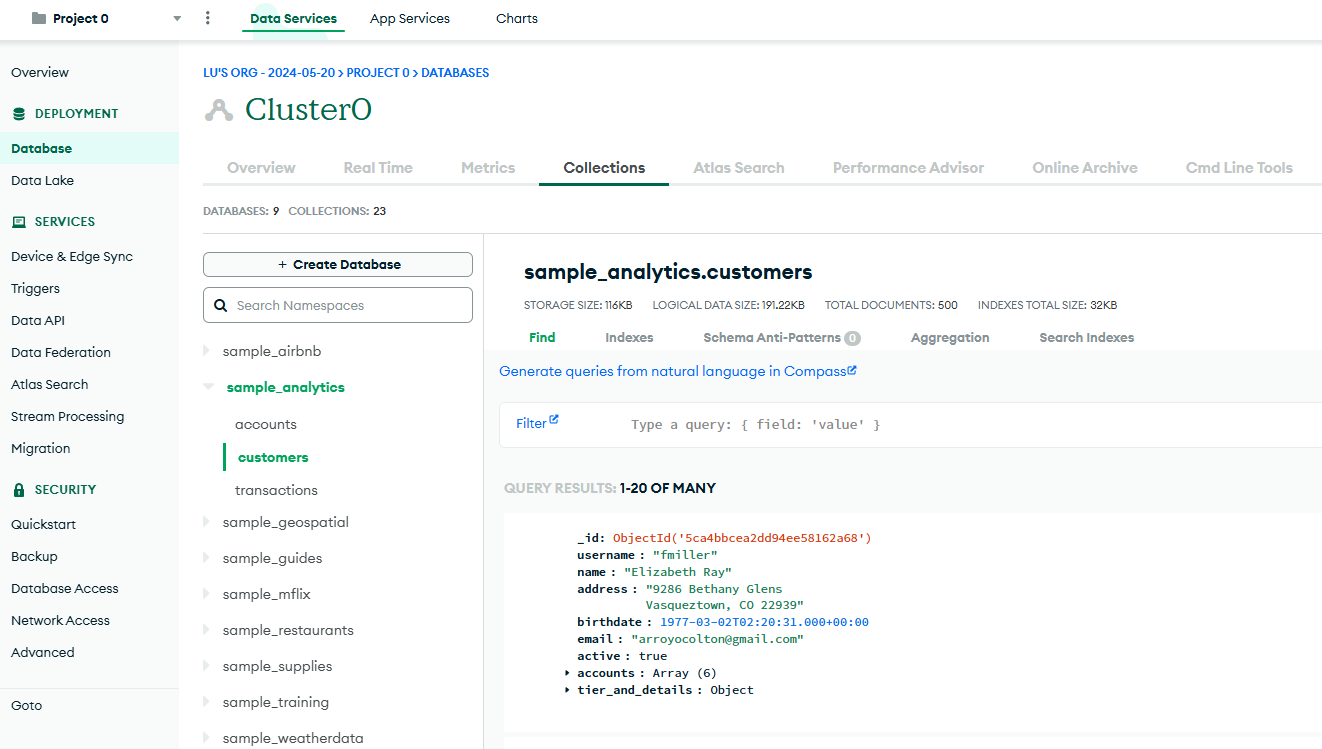
\includegraphics[width=\textwidth]{chapters/part-3/figures/atlas_dashboard_2.png}
	\caption{A demonstration of MongoDB Atlas dashboard where the databases and collections under ``\texttt{Project 0}'', ``\texttt{Cluster0}'' are browsed. Database ``\texttt{sample\_analytics}'', collection ``\texttt{customers}'' is selected. There are $500$ documents under this collection.} \label{ch:database:atlasdashboard2}
\end{figure}











\section{Non-RDB Example: Redis}

Redis, short for \textit{REmote DIctionary Server}, is an open-source in-memory distributed key-value database. It is often used as a lightweight database, cache tool, or message broker. Some key features are listed below.

\begin{itemize}
\item In-memory storage. This speeds up reading and writing operations.
\item Persistence. While primarily it is an in-memory database, it also offers variety of ways to persist data on disk without compromising a lot on performance.
\item Complex data structures and associated atomic operations. Though Redis is key-value store, it supports more complex data structures than that.
\item High availability via replicas.
\item Distributed storage via horizontal partitioning.
\item Lightweight.
\end{itemize}

\section{Non-RDB Example: AllegroGraph}

Graph-based database is elsewhere introduced in details in notebook \textit{A Notebook on Probability, Statistics and Data Science} under semantic web. Check that notebook for more details. 